\documentclass[11pt,letterpaper]{article}

% ── Packages ──────────────────────────────────────────────
\usepackage[margin=1in]{geometry}
\usepackage{amsmath,amssymb}
\usepackage{mathtools}
\usepackage{booktabs}
\usepackage{enumitem}
\usepackage{hyperref}
\usepackage[dvipsnames]{xcolor}
\usepackage{titlesec}
\usepackage{microtype}
\usepackage{parskip}
\usepackage{tikz}
\usetikzlibrary{arrows.meta,positioning,calc,fit}

% ── Formatting ────────────────────────────────────────────
\hypersetup{colorlinks=true, linkcolor=NavyBlue, citecolor=NavyBlue, urlcolor=NavyBlue, pdfstartview=FitH}
\titleformat{\section}{\large\bfseries}{\thesection}{1em}{}
\titleformat{\subsection}{\normalsize\bfseries}{\thesubsection}{1em}{}
\titleformat{\subsubsection}{\normalsize\itshape}{\thesubsubsection}{1em}{}

% ── Math shortcuts ────────────────────────────────────────
\newcommand{\bfp}{\mathbf{p}}
\newcommand{\bfz}{\mathbf{z}}
\newcommand{\bfy}{\mathbf{y}}
\newcommand{\bfd}{\mathbf{d}}
\newcommand{\cS}{\mathcal{S}}
\newcommand{\R}{\mathbb{R}}
\newcommand{\pp}{\,\text{pp}}

\begin{document}

% ── Title ─────────────────────────────────────────────────
\begin{center}
{\LARGE\bfseries Neural Field Perceiver}\\[6pt]
{\large Cross-Patient Speech Decoding from Intra-Operative $\mu$ECoG\\via Spatially-Grounded Electrode Encoding}\\[12pt]
{\normalsize Ben Tang \quad\textbar\quad Greg Cogan Lab, Duke University}\\[4pt]
{\normalsize April 2026 \quad\textbar\quad Version 12}
\end{center}

\medskip\noindent\rule{\textwidth}{0.4pt}\medskip

\noindent Technical design document. \textbf{One idea}: use MNI electrode coordinates to build spatially-grounded cross-patient representations, supervised by an auxiliary electrode reconstruction loss. Everything else is standard machinery.

Claims labeled \textbf{supported}, \textbf{observed}, or \textbf{hypothesis}.
Structural assumptions that could be wrong: \textcolor{BrickRed}{red}.

\tableofcontents
\newpage


%% ====================================================================
%%  SECTION 1: PROBLEM
%% ====================================================================

\section{Problem}\label{sec:problem}

Each patient's $\mu$ECoG array is a sparse spatial sample of cortical high-gamma activity (HGA, 70--150\,Hz, 200\,Hz) during speech. The array sits on left ventral sensorimotor cortex (vSMC), and electrode positions in MNI-152 space are determined post-hoc from surgical reconstruction.

\textbf{Hardware.} LCP thin-film arrays (Dyconex~\cite{duraivel2023}), physically flexible --- they conform to cortical curvature. Two configurations:

\begin{table}[ht!]\centering\small
\begin{tabular}{@{}lll@{}}
\toprule
& \textbf{128-ch (DBS)} & \textbf{256-ch (craniotomy)} \\
\midrule
Grid & $8 \times 16$ & $12 \times 22$ \\
Pitch & 1.33\,mm & 1.72\,mm \\
Footprint & ${\sim}11 \times 21$\,mm & ${\sim}21 \times 38$\,mm \\
Contact diameter & 200\,$\mu$m & 200\,$\mu$m \\
\bottomrule
\end{tabular}
\end{table}

\textbf{Task.} Non-word repetition (intra-operative, no delay --- patients repeat immediately after hearing stimulus): 52 CVC/VCV tokens, 9 phonemes, 3 positions per token. Output: three 9-way classifications per trial. Epochs are per-phoneme, locked to each phoneme's production onset via MFA. We use the production-only window ($t_{\min}{=}0.0$, $t_{\max}{=}1.0$\,s relative to response onset) to exclude auditory activation from the stimulus.

\textbf{Cross-patient challenge.} Arrays are offset 15--25\,mm in MNI space with variable rotation. Channel indices are meaningless across patients. Current LOPO achieves PER\,=\,0.762 (S14, grouped-by-token CV) using a per-patient Conv2d read-in that ignores electrode coordinates entirely. 55 architecture/training experiments converge to PER 0.750--0.780, suggesting a systematic barrier.

\textbf{Constraints.}

\begin{table}[ht!]\centering\small
\begin{tabular}{@{}llr@{}}
\toprule
\textbf{Constraint} & \textbf{Value} & \textbf{Impact} \\
\midrule
Sig.\ electrodes/patient & 63--201 & Sparse cortical sampling \\
Cross-patient offset & 15--25\,mm & Different cortex sampled \\
Trials/patient & 46--178 & Small-data regime \\
Utterance/patient & ${\sim}$1\,min & SSL has failed \\
Patients & ${\sim}$10 & Too few for large models \\
\bottomrule
\end{tabular}
\end{table}

\textbf{Why coordinates might help.} The current pipeline treats each patient's electrode array as an opaque tensor. Per-patient Conv2d learns spatial filters independently per patient --- nothing is spatially shared. If two patients have electrodes sampling the same cortical region, the model cannot exploit this. MNI coordinates make spatial correspondence explicit: electrodes at similar brain positions should carry similar information, regardless of which patient they belong to.


%% ====================================================================
%%  SECTION 2: IDEA
%% ====================================================================

\section{Idea: Spatially-Grounded Electrode Encoding}\label{sec:idea}

\subsection{What we assume}

Speech motor cortex has \textbf{conserved somatotopic organization}: the mapping from brain position to articulatory function is approximately shared across people. Gross somatotopic ordering (medial$\to$lateral: leg$\to$hand$\to$face) is essentially invariant~\cite{roux2020}. Fine structure varies --- speech motor cortex shows the highest positional variability (${\sim}$15--25\,mm~\cite{eichert2020}) and morphological diversity (five distinct sulcal types in the subcentral region). But functional connectivity is the most conserved feature of sensorimotor cortex~\cite{mueller2013}. The spatial map exists; its absolute position varies.

\textcolor{BrickRed}{\textit{Untested:}} That this conservation is strong enough, at $\mu$ECoG resolution, to transfer across $N{=}10$ patients with centimeter-scale positional uncertainty. This is the central empirical question.

\subsection{The three components}\label{sec:components}

The idea has three parts, all spatial:

\begin{enumerate}[leftmargin=2em]
\item \textbf{Spatial tokenization.} Each electrode becomes a token whose spatial identity comes from its MNI coordinates (via Fourier positional encoding), not its channel index.

\item \textbf{Spatial aggregation.} Cross-attention from fixed virtual electrodes to real electrodes, with a distance bias in the attention logits. Electrodes near a virtual electrode contribute more. This maps variable electrode counts to a fixed shared spatial frame.

\item \textbf{Spatial supervision.} An auxiliary loss that reconstructs each electrode's observed activity from the latent representation and the electrode's coordinates. This forces the latent to be spatially meaningful --- if you know \textit{where} an electrode is, you should be able to predict \textit{what} it sees.
\end{enumerate}

These three components are coupled: spatial supervision only makes sense because tokens carry spatial identity, and spatial aggregation is what gives the latent representation a spatial structure to supervise against. Remove any one and the others lose their purpose.

Everything else in the architecture --- temporal attention, classification head, training protocol --- is standard.

\subsection{What the patient-specific components are}

Per patient $i$:
\begin{itemize}[leftmargin=2em]
\item $\Delta^{(i)} \in \R^3$, $\omega^{(i)} \in \R^3$: translation and rotation of MNI coordinates (6 params). Absorbs systematic registration error. L2-regularized ($10^{-3}$), init at $\mathbf{0}$.
\item $e^{(i)} \in \R^{64}$: patient embedding entering \textbf{only} the reconstruction decoder. Absorbs impedance, gain, tissue differences. During training, dropped to $\mathbf{0}$ with $p{=}0.5$ so the decoder learns to reconstruct without patient identity (matching zero-shot test conditions).
\end{itemize}

Total: 70 learnable params per patient. The encoder sees \textbf{no patient identity} --- only electrode coordinates and activity. This forces the latent representation into a patient-agnostic spatial frame.

\textcolor{BrickRed}{\textit{Position leakage:}} At $N{=}10$, each patient's electrode positions trivially identify them. The benefit of withholding $e$ from the encoder is not preventing memorization but improving transfer: position-conditioned processing generalizes to new positions; embedding-conditioned processing does not.


%% ====================================================================
%%  SECTION 3: ARCHITECTURE
%% ====================================================================

\section{Architecture}\label{sec:architecture}

\begin{center}
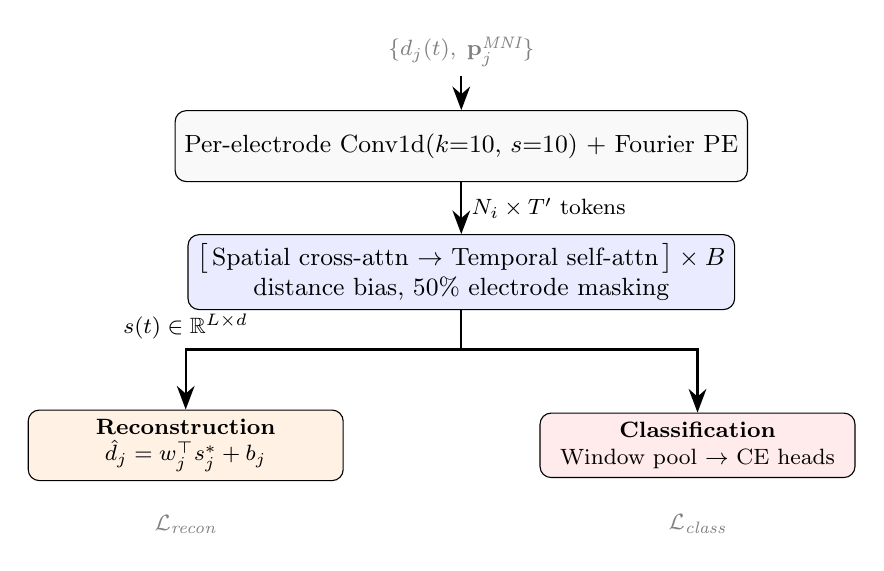
\begin{tikzpicture}[
  box/.style={draw, rounded corners, minimum width=5.5cm, minimum height=0.9cm, align=center, font=\small},
  smallbox/.style={draw, rounded corners, minimum width=4cm, minimum height=0.8cm, align=center, font=\footnotesize},
  arrow/.style={-{Stealth[length=3mm]}, thick},
  label/.style={font=\footnotesize\itshape, text=gray}
]

\node[box, fill=gray!5] (input) at (0, 0.8) {Per-electrode Conv1d($k{=}10$, $s{=}10$) + Fourier PE};

\node[box, fill=blue!8] (block) at (0, -0.8) {$\bigl[$\,Spatial cross-attn $\to$ Temporal self-attn\,$\bigr] \times B$\\distance bias, 50\% electrode masking};

\node[smallbox, fill=orange!10] (obs) at (-3.5, -3.0) {\textbf{Reconstruction}\\$\hat{d}_j = w_j^\top s_j^* + b_j$};

\node[smallbox, fill=red!8] (phoneme) at (3.0, -3.0) {\textbf{Classification}\\Window pool $\to$ CE heads};

\node[label] (raw) at (0, 2.0) {$\{d_j(t),\; \bfp_j^{\text{MNI}}\}$};

\draw[arrow] (raw) -- (input);
\draw[arrow] (input) -- (block) node[midway, right, font=\footnotesize] {$N_i \times T'$ tokens};
\draw[arrow] (block.south) -- ++(0,-0.5) -| (obs.north) node[midway, above, font=\footnotesize] {$s(t) \in \R^{L \times d}$};
\draw[arrow] (block.south) -- ++(0,-0.5) -| (phoneme.north);

\node[label] at (-3.5, -4.0) {$\mathcal{L}_{\text{recon}}$};
\node[label] at (3.0, -4.0) {$\mathcal{L}_{\text{class}}$};

\end{tikzpicture}
\end{center}

\begin{equation}
\boxed{\mathcal{L} = \mathcal{L}_{\text{class}} + \lambda \,\mathcal{L}_{\text{recon}}, \qquad \lambda \in \{0, 0.1, 0.3\}}
\end{equation}


\subsection{Electrode tokens}\label{sec:tokens}

For electrode $j$ on patient $i$, at temporal bin $t'$:
\begin{equation}
\text{token}_j(t') = \underbrace{\text{Conv1d}(d_j;\; k{=}10,\, s{=}10)_{t'}}_{\text{activity (time-varying)}} + \underbrace{\text{Linear}\bigl(\gamma(\tilde{\bfp}_j)\bigr)}_{\text{position (constant)}} + \underbrace{\text{sinPE}(t')}_{\text{temporal index}}
\end{equation}

\textbf{Temporal binning.} Per-electrode Conv1d($1 \to d$, $k{=}10$, $s{=}10$): non-overlapping 50\,ms windows at 200\,Hz $\to$ $T' \approx 20$ tokens. Shared weights across all electrodes and patients. Matches field standard (Spalding, Willett: 20\,Hz effective rate). Our BiGRU experiments show stride\,=\,5 (40\,Hz) $\approx$ stride\,=\,10 (20\,Hz); test as ablation.

\textbf{Fourier PE ($F{=}3$).} Calibrated MNI coordinates $\tilde{\bfp}_j = R(\omega^{(i)}) \bfp_j + \Delta^{(i)}$, standardized so the speech motor region spans $[-1, 1]$ per axis:
\begin{equation}
\gamma(\bar{\bfp}) = \bigl[\sin(2^0 \pi \bar{\bfp}),\; \cos(2^0 \pi \bar{\bfp}),\; \ldots,\; \sin(2^{2} \pi \bar{\bfp}),\; \cos(2^{2} \pi \bar{\bfp})\bigr] \in \R^{18}
\end{equation}
Wavelengths: 30\,mm (full-array), 15\,mm (articulatory region), 7.5\,mm (sub-region). Projected via Linear($18 \to d$).

\textbf{Why $F{=}3$.} Intraoperative MNI coordinates carry ${\sim}5$--$10$\,mm RMS error from stacking sources (navigation 2--4\,mm, brain shift 2--10\,mm, normalization 2--3\,mm). The finest wavelength at $F{=}3$ is 7.5\,mm --- just above the noise floor. $F{=}4$ (3.75\,mm) would encode noise.

\textbf{Geometric calibration} ($\Delta^{(i)}, \omega^{(i)}$, 6 params/patient). The registration system performs one calibration per patient; that systematic bias propagates to all electrodes. Rigid correction absorbs this dominant error mode. Non-rigid brain shift (${\sim}2$--$10$\,mm, spatially smooth) is handled by soft attention --- a few mm of position error still places electrodes in approximately the correct virtual electrode neighborhood.


\subsection{Virtual electrodes}\label{sec:virtual-electrodes}

$L = 16$ query vectors at \textbf{fixed} MNI positions, with learned query content vectors. Each virtual electrode asks ``what is the neural activity near this brain position?'' via cross-attention to all real electrodes. Output: $s(t) \in \R^{L \times d}$ --- a fixed-size spatial representation regardless of electrode count.

\textbf{Why virtual electrodes.} Patient A has 63 electrodes; Patient B has 201, at different positions. The downstream decoder needs a fixed-size input that means the same thing across patients. Virtual electrodes provide this: they query the brain at the \textbf{same 16 anatomical positions} for every patient, and the soft attention handles the fact that different real electrodes are nearby for each patient.

\textbf{Positions.} Fixed at Brainnetome atlas~\cite{fan2016} centroids of speech motor subregions (lip M1, tongue M1, jaw M1, laryngeal M1, lip S1, tongue S1, ventral premotor, SMA, etc.). Not learned --- at $N{=}10$, the atlas (derived from hundreds of subjects) is a better population average than anything gradient descent could find. Inter-patient anatomical variability (${\sim}15$--$25$\,mm) and MNI error (${\sim}5$--$10$\,mm) are both handled by the \textbf{soft spatial attention}, not by moving query positions: the Gaussian distance bias decays smoothly, so a virtual electrode at ``atlas tongue M1'' still attends to real electrodes 10--15\,mm away. Spacing: ${\sim}5$\,mm, matching somatotopic scale.


\subsection{Spatiotemporal blocks ($\times B$)}\label{sec:blocks}

Each block alternates:

\textbf{(a) Spatial cross-attention} (per time bin). Virtual electrodes (Q) attend to real electrode tokens (K, V):
\begin{equation}
A_{ij} = \frac{Q_i \cdot K_j}{\sqrt{d_h}} \;-\; \alpha_h \cdot \|\bar{\bfp}_i - \bar{\bfp}_j\|^2
\end{equation}
Standard scaled dot-product attention plus a learnable isotropic distance bias $\alpha_h > 0$ per head (4 heads, init 1.0). The distance term makes attention spatially local by default; content similarity can override for distant but functionally related electrodes.

\textbf{(b) Temporal self-attention} (per virtual electrode). Each of 16 virtual electrodes attends across ${\sim}20$ time bins. 4 heads, sinusoidal temporal PE. Captures articulatory dynamics.

\textbf{Block internals.} Pre-LN residual connections, ReLU FFN ($d_\text{ff} = 4d$), dropout $p{=}0.2$, DropPath $p{=}0.1$.

\textbf{Electrode masking.} During training, 50\% of electrodes are excluded from KV for all time steps. The reconstruction loss is still computed at masked positions, forcing spatial interpolation.


\subsection{Reconstruction decoder}\label{sec:recon-decoder}

Predicts each electrode's activity from the latent state and the electrode's position.

\textbf{Position-weighted aggregation.} Electrode $j$ gets a local latent vector by weighting virtual electrode outputs by spatial proximity:
\begin{equation}
s_j^*(t) = \sum_{\ell=1}^{L} \text{softmax}_\ell\!\bigl(-\alpha_{\text{dec}} \|\bar{\tilde{\bfp}}_j - \bar{\text{v}}_\ell\|^2\bigr) \cdot s_\ell(t)
\end{equation}

\textbf{Prediction.} Linear projection per time bin:
\begin{equation}
\hat{d}_j^{(i)}(t) = w(e^{(i)}, \tilde{\bfp}_j)^\top s_j^*(t) + b(e^{(i)}, \tilde{\bfp}_j)
\end{equation}
where $w, b$ come from a small MLP($[\tilde{\bfp}_j;\; e^{(i)}] \to \R^{d+1}$), 2 layers, ${\sim}$5K params total. During training, $e^{(i)} \to \mathbf{0}$ with $p{=}0.5$.

\textbf{Reconstruction loss.}
\begin{equation}
\mathcal{L}_{\text{recon}} = \frac{1}{N_i T'} \sum_{j,t'} \bigl(d_j(t') - \hat{d}_j(t')\bigr)^2
\end{equation}
Computed over all electrodes including masked ones. Gradient flows back through the encoder, providing the spatial supervision signal.


\subsection{Phoneme decoder}\label{sec:phoneme-decoder}

Mean-pool across $L$ virtual electrodes: $s_\text{pool}(t') = \frac{1}{L}\sum_\ell s_\ell(t')$.

\textbf{Temporal readout.} The data provides per-phoneme MFA epochs, but MFA alignment is unreliable for ${\sim}50\%$ of patients (300--500\,ms offsets observed). We therefore use \textbf{full-trial input} ($t_\text{min}{=}0.0$, $t_\text{max}{=}1.0$\,s, all 3 phonemes in one sample) with learned temporal attention queries --- one per phoneme position --- matching our current pipeline:
\begin{equation}
\bfz_p = \sum_{t'} \text{softmax}_{t'}\!\bigl(q_p \cdot s_\text{pool}(t') / \sqrt{d}\bigr) \;\cdot\; s_\text{pool}(t'), \qquad p \in \{1,2,3\}
\end{equation}
Each $q_p \in \R^d$ is a learned query. Position 1's query learns to attend to early frames, position 3's to late frames. This handles unequal phoneme durations without relying on MFA boundaries. Validated at PER\,=\,0.737 (per-patient, S14).

Per position, dual head:
\begin{equation}
\text{logits}_p = \frac{1}{2}\bigl(\text{Linear}(\bfz_p \to 9) + \tau \cdot \text{normalize}(\text{Linear}(\bfz_p \to 15)) \cdot A^\top\bigr)
\end{equation}
$A \in \R^{9 \times 15}$: fixed articulatory feature matrix. $\tau$: learnable temperature.

$\mathcal{L}_\text{class} = \frac{1}{3}\sum_p \text{FocalCE}(\text{logits}_p, y_p;\; \gamma{=}2,\; \text{LS}{=}0.1)$ with mixup ($\alpha{=}0.2$).


\subsection{Parameter budget}

\begin{table}[ht!]\centering\small
\begin{tabular}{@{}lrll@{}}
\toprule
\textbf{Module} & \textbf{Params} & \textbf{Shared?} & \textbf{Note} \\
\midrule
Conv1d($1 \to d$, $k{=}10$) & ${\sim}$0.7K & Shared & Temporal binning \\
Fourier PE + Linear & ${\sim}$1.2K & Shared & Spatial encoding \\
Blocks ($\times B$) & ${\sim}100B$K & Shared & The bulk \\
\quad distance scales $\alpha_h$ & $4B$ & Shared & \\
\quad virtual positions & 48 & Fixed & Atlas (not learned) \\
Reconstruction decoder & ${\sim}$5K & Shared & Position-aware linear \\
Phoneme heads ($\times 3$) & ${\sim}$5K & Shared & Dual CE + artic \\
\midrule
$\Delta^{(i)} + \omega^{(i)}$ & 6/pt & Per-patient & Registration correction \\
$e^{(i)}$ & 64/pt & Per-patient & Decoder only \\
\midrule
\textbf{Total ($B{=}1$)} & $\mathbf{{\sim}112}$\textbf{K} & & Comparable to current BiGRU \\
\textbf{Total ($B{=}2$)} & $\mathbf{{\sim}212}$\textbf{K} & & $1.8\times$ current \\
\bottomrule
\end{tabular}
\end{table}

\textcolor{BrickRed}{\textit{Capacity concern:}} 112--212K params on ${\sim}$1,300 trials. Mitigated by: electrode masking (50\%), reconstruction loss (${\sim}2.6$M targets vs.\ 3.9K classification labels), dropout, early stopping. $B{=}1$ is the safe default; $B{=}2$ only if $B{=}1$ underfits.


%% ====================================================================
%%  SECTION 4: TRAINING
%% ====================================================================

\section{Training and Evaluation}\label{sec:training}

\subsection{Phase 1: Source training}

$N{-}1$ source patients. AdamW ($10^{-3}$), geometric params ($\Delta, \omega$, virtual positions) at $3 \times 10^{-4}$. Cosine decay with 20-epoch warmup. Weight decay $10^{-4}$, grad clip 5.0, batch 16. Early stopping on 20\% held-out source validation, patience 7.

\subsection{Phase 2: Target adaptation}

Per fold of 5-fold grouped-by-token CV on target patient:
\begin{enumerate}[leftmargin=2em]
\item \textbf{Linear probe.} Freeze encoder. Train decoder + $\Delta^{(\text{tgt})} + \omega^{(\text{tgt})} + e^{(\text{tgt})}$. 150 epochs.
\item \textbf{Fine-tune.} Unfreeze encoder at $0.1\times$ LR. 100 epochs, patience 7.
\end{enumerate}

\subsection{Evaluation}

\textbf{Zero-shot:} Phase 1 only, $\Delta{=}\omega{=}e{=}\mathbf{0}$. Pure coordinate generalization.

\textbf{LP-FT (primary):} Phase 1 $\to$ Phase 2. Matches clinical calibration.

\textbf{Metrics:} PER (edit distance), grouped-by-token 5-fold CV, 3 seeds. Full recipe: weighted $k$-NN ($k{=}10$), TTA 16, dual head.


%% ====================================================================
%%  SECTION 5: ABLATIONS
%% ====================================================================

\section{Ablation Plan}\label{sec:ablations}

The ablation structure isolates each component of the spatial idea:

\begin{table}[ht!]\centering\small
\begin{tabular}{@{}clp{7cm}@{}}
\toprule
\textbf{ID} & \textbf{Ablation} & \textbf{What it tests} \\
\midrule
A1 & Current Conv2d+BiGRU & Anchor baseline (PER ${\sim}$0.76) \\
A2 & Perceiver, no coordinates & Architecture benefit alone (A2 vs A1) \\
A3 & + Fourier PE on MNI coords & Coordinate benefit (A3 vs A2) \\
A4 & + reconstruction loss & Spatial supervision benefit (A4 vs A3) \\
A5 & + $\Delta/\omega$ calibration & Calibration benefit (A5 vs A4) \\
A6 & Random MNI positions & Sanity: real coords $>$ random (A6 vs A3) \\
\midrule
A7 & Population-level (all patients) & Is the 0.76 wall S14-specific? \\
A8 & $\lambda \in \{0, 0.1, 0.3, 0.5\}$ & Reconstruction weight sweep \\
A9 & $L \in \{4, 8, 16, 32\}$ & Virtual electrode count \\
A10 & $B \in \{1, 2\}$ & Block count / capacity \\
A11 & $F \in \{2, 3, 4\}$; Linear PE & PE resolution \\
A12 & $e$ in encoder vs decoder-only & Patient identity split \\
A13 & Cross-task data (Duraivel 2025) & Data quantity vs architecture \\
\bottomrule
\end{tabular}
\end{table}

\textbf{A1--A6 are the core experiment.} Each row adds exactly one component. If A3 $\approx$ A2, coordinates don't help and the paper's hypothesis is wrong. If A4 $\approx$ A3, reconstruction loss doesn't help and we drop it. Clean isolation.


%% ====================================================================
%%  SECTION 6: PRIORITIES AND RISKS
%% ====================================================================

\section{Priorities and Risks}\label{sec:priorities}

\subsection{Priority ordering}

\begin{enumerate}[leftmargin=2em]
\item \textbf{Cross-task data pooling (A13).} Lowest risk. Same phonemes, overlapping patients~\cite{duraivel2025}. Directly addresses data scarcity. Works with any architecture.

\item \textbf{Population-level evaluation (A7).} Methodology fix. Required to know if we have a real effect.

\item \textbf{Coordinate architecture (A1--A6).} Highest novelty, highest risk. The central bet.
\end{enumerate}

\subsection{Hard gate}

All MNI-dependent claims require extracting and auditing electrode coordinates from BioImage Suite (DBS) / Brainlab (craniotomy). If coordinates are unavailable or too noisy, the fallback is A2 (Perceiver on scaled grid positions with no MNI).

\subsection{Success criteria}

\textbf{Primary:} Population mean PER improves $\geq 3\pp$ over Conv2d+BiGRU baseline, $\geq 3$ seeds, paired Wilcoxon $\alpha{=}0.05$.

\textbf{Mechanistic:} A3 $>$ A2 (coordinates help). A4 $>$ A3 (reconstruction helps). Learned $\Delta^{(i)}$ magnitudes consistent with known registration error ($< 15$\,mm).

\subsection{Risks}

\begin{table}[ht!]\centering\small
\begin{tabular}{@{}p{0.35\textwidth}cp{0.40\textwidth}@{}}
\toprule
\textbf{Risk} & \textbf{Severity} & \textbf{Mitigation} \\
\midrule
MNI coordinates unavailable & High & Fall back to A2 (grid positions) \\
MNI too noisy ($>10$\,mm) & High & $\Delta/\omega$ calibration; $F{=}2$ \\
Recon competes with classification & Med & $\lambda$ sweep (A8); $\lambda{=}0$ \\
212K params overfits 1{,}300 trials & Med & $B{=}1$ (112K); masking; early stop \\
Coords don't help (A3 $\approx$ A2) & Med & Paper becomes ``Perceiver for uECOG'' \\
\bottomrule
\end{tabular}
\end{table}


%% ====================================================================
%%  SECTION 7: DATA
%% ====================================================================

\section{Available Data}\label{sec:data}

\begin{table}[ht!]\centering\small
\begin{tabular}{@{}lllcc@{}}
\toprule
\textbf{Cohort} & \textbf{Patients} & \textbf{Trials} & \textbf{MNI?} & \textbf{Usage} \\
\midrule
PS (Spalding published) & 8 & ${\sim}$1096 & Expected$^*$ & Source / target \\
PS (additional) & S16, S57 & ${\sim}$250 & Expected$^*$ & Source \\
Cross-task (Duraivel 2025) & 3 overlapping & 156--208/pt & Expected$^*$ & A13 \\
\midrule
\textbf{Total unique PS} & \textbf{10} & $\mathbf{{\sim}1350}$ & & \\
\bottomrule
\end{tabular}
\end{table}

$^*$MNI from BioImage Suite / Brainlab on Box. Extraction and audit required before any coordinate experiments.


% ── Bibliography ──────────────────────────────────────────
\begin{thebibliography}{99}\raggedright

\bibitem{duraivel2023}
Duraivel, S., et al.\ (2023).
High-resolution neural recordings improve the accuracy of speech decoding.
\textit{Nature Communications}, 14, 6938.

\bibitem{duraivel2025}
Duraivel, S., et al.\ (2025).
Distinct neural processes link speech planning and execution.
\textit{bioRxiv}. doi:10.1101/2024.10.07.617122

\bibitem{roux2020}
Roux, F.-E., et al.\ (2020).
The human motor cortex somatotopy.
\textit{The Journal of Physiology}, 598(23), 5301--5316.

\bibitem{eichert2020}
Eichert, N., et al.\ (2020).
Morphological and functional variability in central and subcentral motor cortex.
\textit{Brain Structure and Function}, 226, 263--279.

\bibitem{mueller2013}
Mueller, S., et al.\ (2013).
Individual variability in functional connectivity architecture of the human brain.
\textit{Neuron}, 77(3), 586--595.

\bibitem{fan2016}
Fan, L., et al.\ (2016).
The Human Brainnetome Atlas.
\textit{Cerebral Cortex}, 26(8), 3508--3526.

\end{thebibliography}

\end{document}
